\Section{Introduction}

Computers are present in virtually every aspect of our lives:
middle-schoolers and grandmothers alike use them at home, at school,
and at work. Sadly, computers are mostly used for activities like word
processing, web browsing, e-mail, and games. To truly take advantage
the power of their computers, {\em end-users} must be able to write
programs. This makes end-user programming languages and environments
an important area of research.

A number of end-user programing systems have been proposed.
These systems have focused on various goals, and can be
classified based on several criteria.  One such criterion is the {\em
steepness of the learning curve} --- in other words, how easy it is for
a new user to become productive.  In systems like
Viscuit~\cite{yh03viscuit} and StageCast~\cite{dcs00stagecast}, for
example, simple graphical pattern-matching and rewrite rules allow
end-users to compose simple animations quickly and easily, with very
little training required.

Another criterion is the {\em ceiling height}, i.e., how well the language scales to more complex
problems. A full-fledged programming language with many built-in
features, where the user writes textual programs, will get the highest
marks on this criterion.

  The tension between these criteria makes the task of designing an end-user
programming system a difficult one.
No system that we are aware of has both a gentle
learning curve {\em and} a high ceiling.  Existing systems tend to
spread on the spectrum from gentle learning curve/low ceiling to
steep learning curve/high ceiling.  Viscuit, for example, has a
very low learning curve, but expressions in Viscuit are represented
solely iconically; Viscuit, in fact, does not even have the concept of
numbers or arithmetic.  In such systems, one quickly hits the rather
low ceiling, after initially enjoying simple and easy programs.

  Systems like Scratch~\cite{mbkrsr04@scratch} offer graphical building blocks
that the user can manipulate and combine
with the mouse to construct programs.  The blocks are symbolic
representations of the elements of a program (such as numbers, symbols, and control structures) so the user
has to learn what each block does and means, but as he learns more
about these blocks, his productivity increases.
Unfortunately, this gentle learning curve has some negative
consequences; for example, Scratch intentionally omits the concept of inter-object
reference to avoid confusion.  This design choice makes it
tricky to write a program where multiple objects work together.

  At the other end of the spectrum, there are languages and systems
with fully textual code.  Many educational and end-user development
environments are based on Java, Python and other conventional
languages, which makes them very expressive.  Also, text-based
programming tends to be more efficient than tiles as programs grow in complexity.
{\em Processing}~\cite{rf07processing} and J0~\cite{j0} are based on
simplified versions of Java, and provide end-user-oriented
development environments.  However, users have to deal with syntax
errors, and face a steeper learning curve.

\begin{figure}[tp]
\centering
\scalebox{0.4}{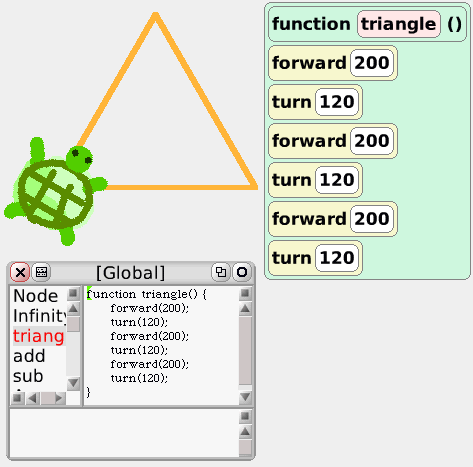
\includegraphics{turtle.eps}}
\caption{A screenshot from the TileScript system.  The smae code is shown as tiles and text-based code.}
\label{fig:turtles}
\end{figure}

\SubSection{The Goal}
  Our goal is to create a new end-user scripting language with a gentle learning
curve and a high ceiling.  Our system should support both tile scripting and
textual coding, and the transition between these two representations should be as
smooth as possible.  Specifically, we aim to make it possible for the user to:
\begin{itemize}
\item
  convert a tile script into equivalent textual code, and vice-versa;
\item
  extend the system by creating new kinds of tiles (abstractions), and optionally customize
  their appearance. (The meaning of new tiles should be described using
  tiles or textual code.)
\item
  ``pop the hood'' of any part of the system, so that he can learn about (and perhaps even modify) it.
\end{itemize}
Although users will most likely get started using the tile scripting interface, all
of the
knowledge they acquire with the tiles will still be valid
once they make the transition to text-based programming.

  Our idea draws upon Squeak
Etoys~\cite{ack97Etoys}\cite{bjkr03PowerfulIdeas}.  Etoys, like Scratch,
offers visual building blocks (called ``tiles'') which the user can
combine by dragging-and-dropping to make a unit of program called
a {\em script}.

\begin{figure}[tp]
\centering
\scalebox{0.4}{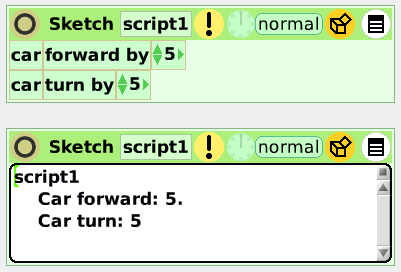
\includegraphics{etoystiles.eps}}
\caption{The same Etoys script in graphical representation and textual representation.}
\label{fig:etoys tiles}
\end{figure}

Etoys tile scripts can be converted into textual code (represented in the system's base language,
Squeak Smalltalk), as shown in Figure~\ref{fig:etoys tiles}.
Unfortunately, this conversion
is only ``one way''; once the user edits the code
textually, there is no mechanism to convert the edited text back to
tiles.
This limitation exists because Smalltalk is a lot more expressive than the tile language, which
makes it is possible for the user to type in code that does not have a
corresponding graphical tile representation.
Also, the Etoys object model is not the same as Smalltalk's, which means that 
the knowledge of the model the user acquires by using Etoys cannot be
translated to Smalltalk programming.
Lastly, because Etoys tiles are implemented in Smalltalk by the system's developers, the end-user is
cannot extend the tile language with new tiles; he is limited to using the ones provided by the
developers.

\begin{figure}[tp]
\centering
\scalebox{0.7}{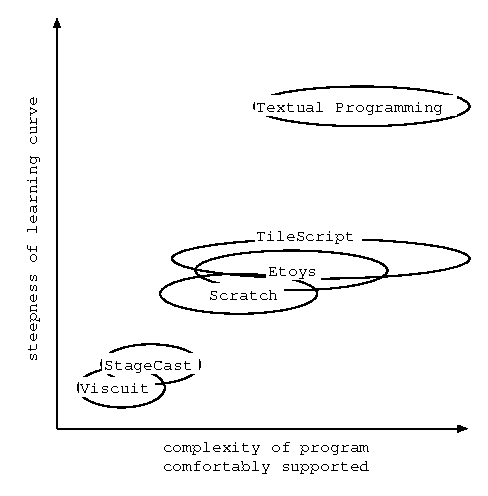
\includegraphics{spectrum.eps}}
\caption{A classification of various end-user programming systems.}
\label{fig:spectrum}
\end{figure}

%% \SubSection{Problems for Providing Extensibility and Openness}

%%   There is another axis in our classification of end-user programming
%% systems; it is {\em extensibility} of the system.  Most of the
%% end-user systems typically provide pre-made, fixed features (such as
%% the matching rules in Viscuit and StageCast, blocks and tiles in
%% Scratch and Etoys, or the Java API in Java).  The Etoys system lets
%% the user create a new script, and the script can be used as a command
%% tile similar to the built-in ones.  However, this is as far as the user
%% can go; the code behind creation of a script is written in Smalltalk
%% by developers who have deep knowledge of the structure of classes.

%%   In visual pattern-matching languages, it is not even conceivable
%% for the user to define new kinds of matching rules.  In the environment
%% for a textually-coded programming language, adding a method or defining
%% a class (for example) is easy, but the system is not usually opened to
%% the end-user, so that defining a new control structure, for example. is usually not
%% possible.

%%   For better educational value, we contend that the entire system
%% should be at least visible to the user.  And it is also desirable that
%% the user be allowed to modify the system, based on an easy to understand model.
%% This almost implies that the entire system should be made of the same
%% thing, and that on top of it we should simply provide good interfaces suited to various end-users for various purposes.
  Figure \ref{fig:spectrum} shows a comparison of the systems described in this section.
In the figure, the vertical axis
denotes the steepness of learning curve; the lower the oval is located,
the easier to start using.  The horizontal axis denotes the complexity
of programs one can write {\em comfortably} in the system.  Our proposed 
system in the middle has similar steepness of learning curve as
Etoys but trys to cover wider kind of programs.

\SubSection{Approach}

  We chose to use JavaScript~\cite{ecma99javascript} as the basis for {\em TileScript} both because
of its simple object model and good reflective facilities, and because we had already produced our own
implementation in Squeak.

  Building our system on top of Squeak gave us access to the Morphic graphics
framework~\cite{jm02MorphicNuBlue}, which facilitated the creation of our tile-based
user interface and gave us access to a rich library of graphical objects.

  We extended our JavaScript implementation with a simple macro system.
TileScript's user-defined tiles are implemented as macros; since
macros are also part of our base language, they can be written using
tiles as well as textual code.

  TileScript programs are stored as parse trees.
We implemented conversions from textual code and tiles to parse trees,
and from parse trees to textual code and tiles.
Thus, tiles and textual code are views of the same model.

  Lastly, we provided a mechanism that allows users to customize the
visual appearance of new as well as existing tiles.

  Figure~\ref{fig:turtles} shows a screenshot from the system.  The
function that draws a triangle is shown in tiles on the right and in
text at the bottom in a JavaScript object inspector.

  The rest of this paper is organized as follows.  Section~\ref{sec:js}
briefly describes our JavaScript implementation and our extensions to the language.
Section~\ref{sec:tile implementation} describes our extensible tile-based programming interface.
In section \ref{sec:discussion}, we discuss the findings from
this experiment.
Section~\ref{sec:related} discusses related work.
Section~\ref{sec:conclusions} discusses future work and concludes.
